%!TEX root = ../../../report.tex
\section{Assembly} % (fold)
\label{sec:assembly}
Due to all basically all the parts have been somehow connected with a 3D printed parts, and all the tolerances of these have been adjusted individually, the assemble process is easy and fast.
The mounting processes has shown to be rapid enough to change some of the parts, as the springs, within minutes.
Furthermore, if any part breaks its creation and replacements is easy enough to reduce the maintenance time enough to consider it as one of the main points of the whole platform.
In the figure \ref{fig:photo_robot_walking}, the complete robot assembled is shown while in the figure \ref{fig:photo_dacbot}, a size comparison between the Dacbot \cite{dacbot1} and RuBi can be done.

\begin{figure}[ht!]
    \centering
    \begin{subfigure}[b]{0.49\textwidth}
        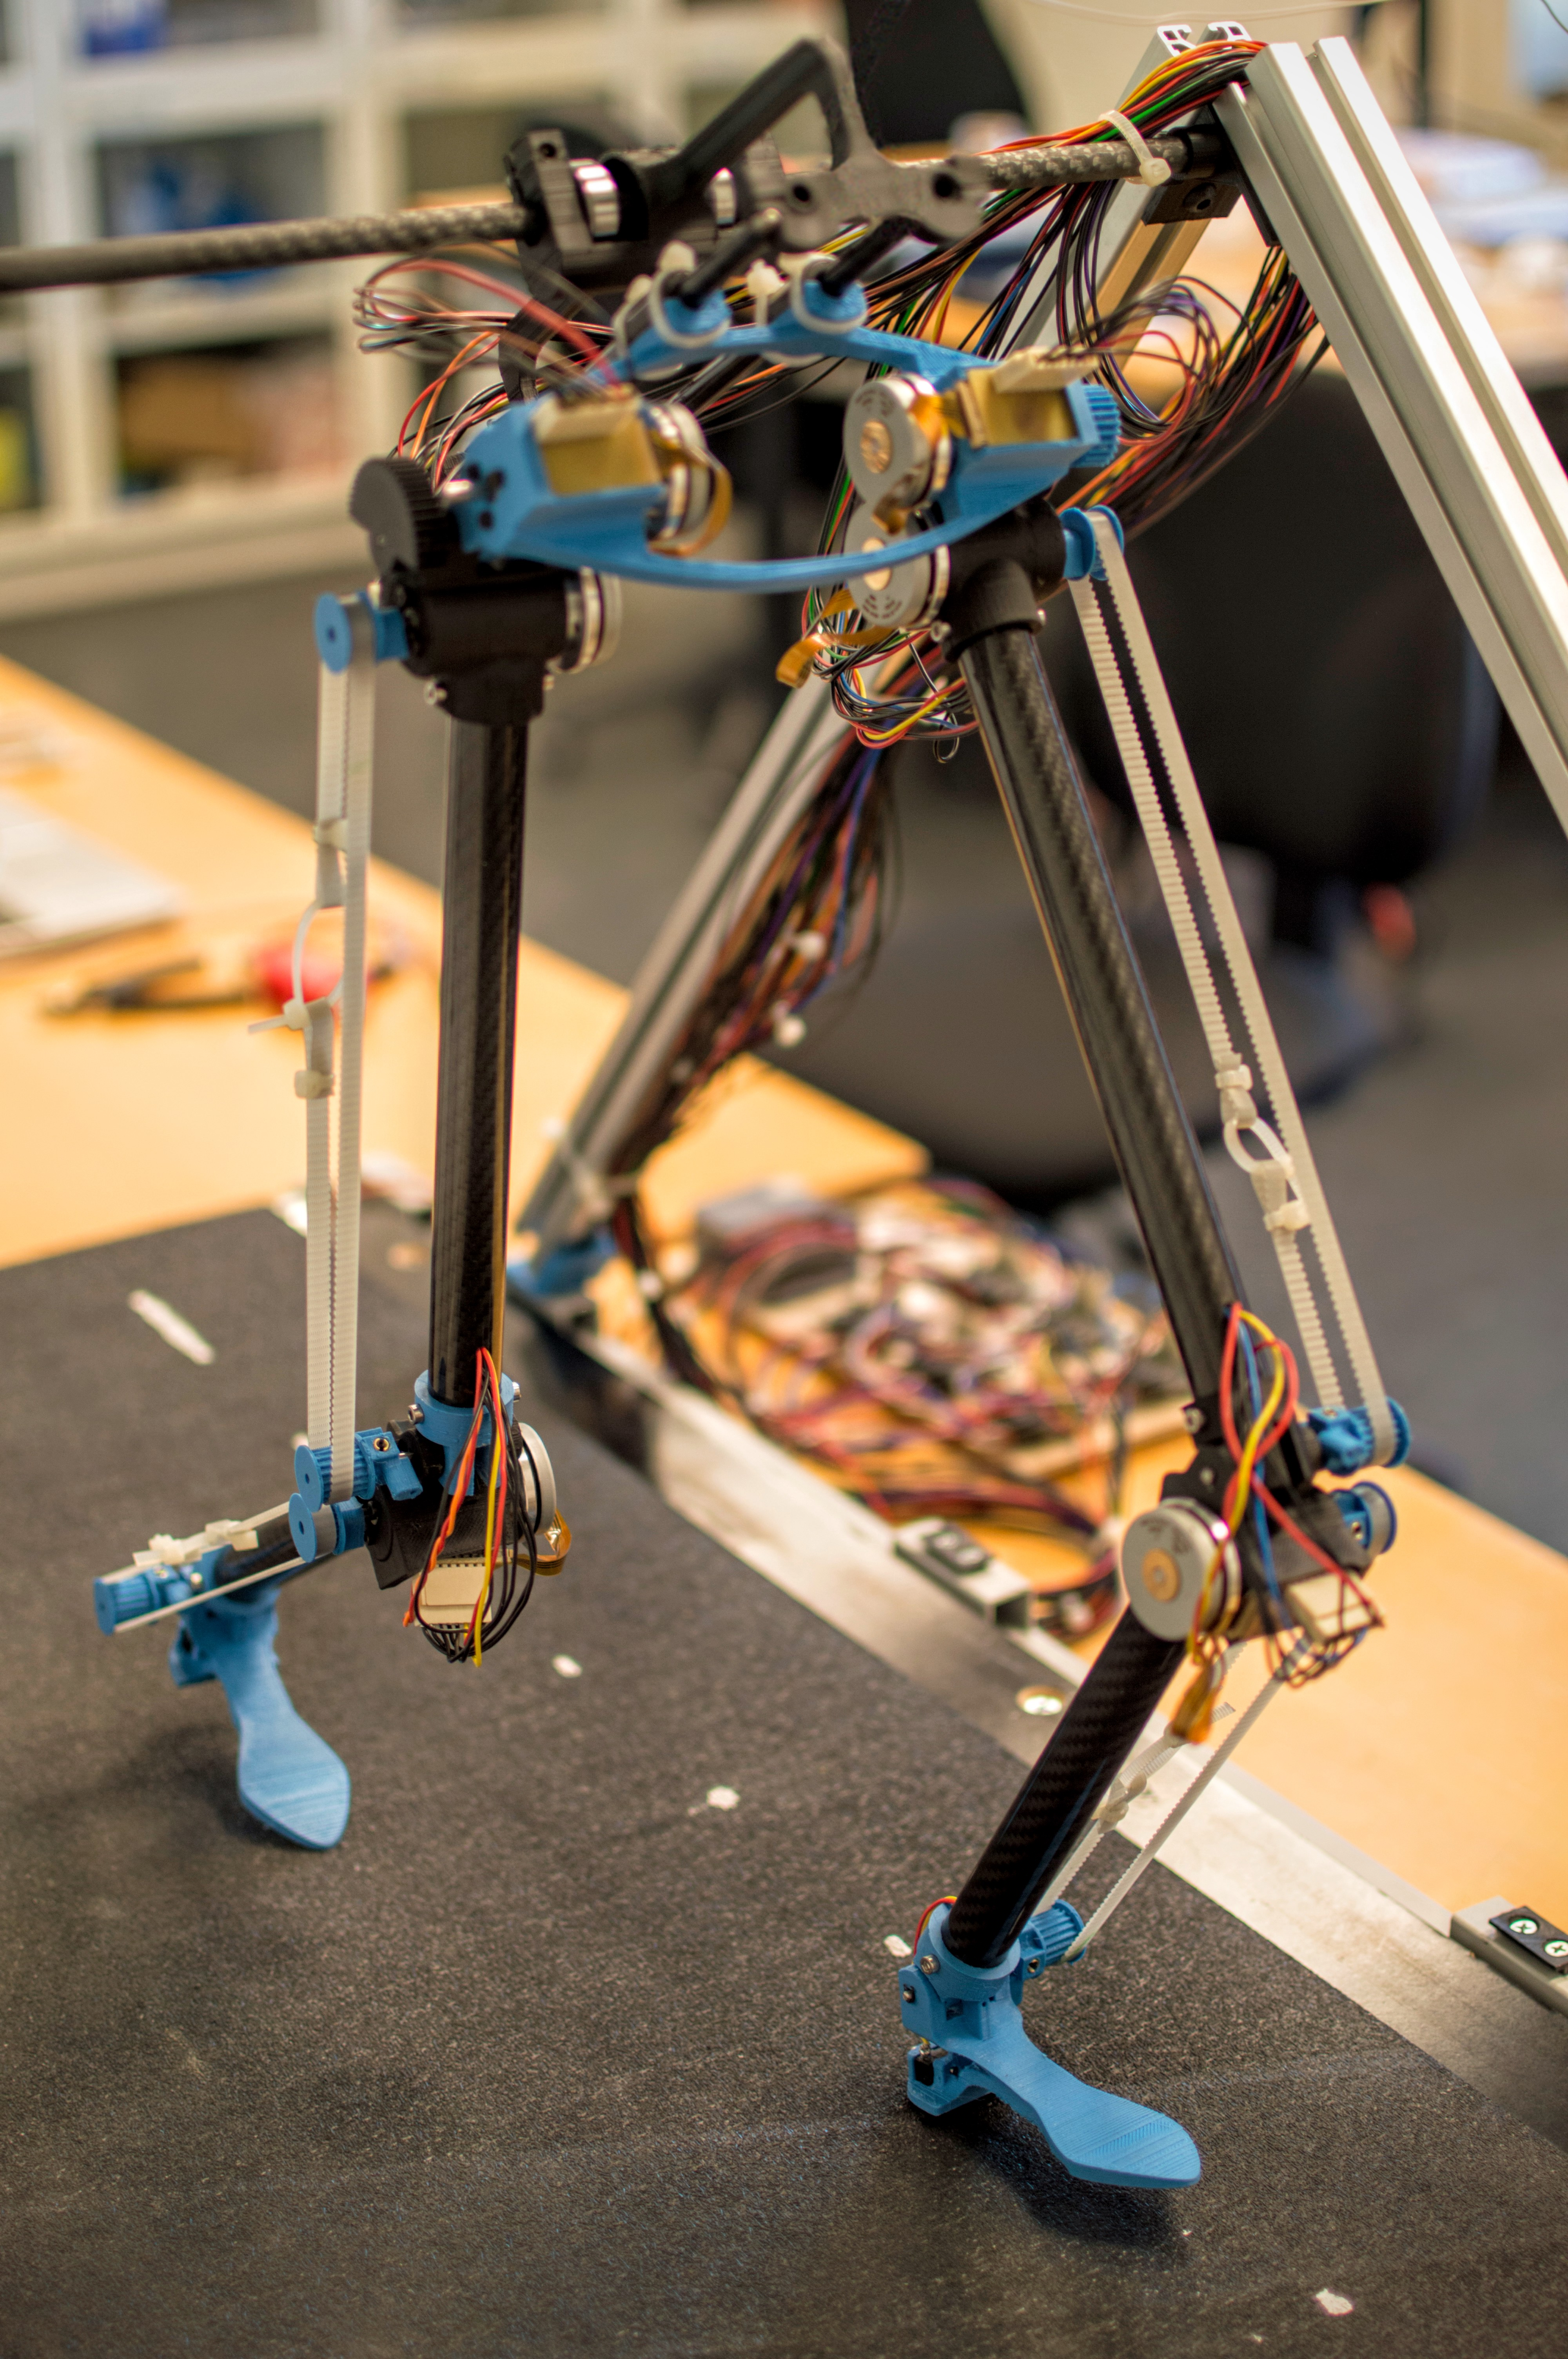
\includegraphics[width=\textwidth]{figures/photo_robot_walking.jpg}
        \caption{RuBi assembled}
        \label{fig:photo_robot_walking}
    \end{subfigure}
    \begin{subfigure}[b]{0.49\textwidth}
        \includegraphics[width=\textwidth]{figures/photo_dacbot.jpg}}
        \caption{RuBi and Dacbot over the same treadmill}
        \label{fig:photo_dacbot}
    \end{subfigure}
\end{figure}    


% section assembly (end)